\documentclass[conference]{IEEEtran}
\IEEEoverridecommandlockouts
\usepackage{cite}
\usepackage{amsmath,amssymb,amsfonts}
\usepackage{algorithmic}
\usepackage{graphicx}
\usepackage{textcomp}
\usepackage{xcolor}
\usepackage{booktabs}
\usepackage{multirow}
\usepackage{balance}
\usepackage[hidelinks]{hyperref}
\usepackage[noabbrev,nameinlink]{cleveref}

% Use IEEE-style reference names with clickable prefixes (e.g., "Fig. 1", "Table I").
\crefname{figure}{Fig.}{Figs.}
\Crefname{figure}{Fig.}{Figs.}
\crefname{table}{Table}{Tables}
\Crefname{table}{Table}{Tables}

\def\BibTeX{{\rm B\kern-.05em{\sc i\kern-.025em b}\kern-.08em
    T\kern-.1667em\lower.7ex\hbox{E}\kern-.125emX}}
\begin{document}

\title{PTM Prediction Using Prot-Mamba}

\author{\IEEEauthorblockN{Harsh Chauhan}
\IEEEauthorblockA{M.S. in Computer Science (Student)\\
Rochester Institute of Technology (RIT)\\
hc3725@g.rit.edu}
}

\maketitle

\begin{abstract}
Post-translational modification (PTM) site prediction is a core task in computational proteomics, where sequence context around candidate residues determines whether a modification is likely to occur. In this project, we develop a two-stage framework for binary PTM classification using fixed-length sequence windows. First, contextual protein representations are extracted from a pretrained PTM-Mamba model for each sample, producing a standardized $51 \times 768$ embedding per sequence window. Second, these embeddings are used to train hybrid deep classifiers based on convolutional and recurrent layers, specifically CNN+GRU and CNN+BiLSTM variants. A structured hyperparameter search is conducted over model family and layer depth. While initial analytical exploration spanned multiple PTMs, the complex deep hybrid models have currently been executed exclusively on the acet\_k dataset. Experimental results on this acet\_k task show that CNN+GRU achieves the strongest validation performance among tested configurations, with validation MCC around 0.5019 and F1 around 0.75 in the best run. The study demonstrates that combining pretrained protein language model embeddings with lightweight sequence classifiers yields a stable and scalable PTM prediction pipeline suitable for extension across PTM types.
\end{abstract}

\begin{IEEEkeywords}
post-translational modification, deep learning, protein language models, proteomics, bioinformatics, acetylation
\end{IEEEkeywords}

\section{Introduction}

Post-translational modifications (PTMs) are biochemical mechanisms in which cells covalently attach functional groups or proteins to specific amino acid residues, fundamentally altering their physical and chemical properties \cite{zhong2023ptm}. By modifying proteins after their primary synthesis, PTMs multiply the complexity and functionality of the cellular proteome without requiring de novo gene expression. This introduces a highly dynamic and responsive regulatory layer that dictates critical biological processes such as signaling cascades, cell cycle progression, protein stability, and localization \cite{li2022dbptm}.

\subsection{Computational Challenge}
Mass spectrometry (MS) remains the gold standard experimental technique for identifying PTMs and localizing modification sites across the proteome. While MS technologies have seen revolutionary advances in resolution and throughput, they suffer from practical and fundamental limitations \cite{messner2023mass}. Modifications like acetylation can be highly transient or exist at substoichiometric levels within the cellular pool, causing them to fall below detection thresholds. Furthermore, biochemical enrichment methods intended to magnify PTM signals often introduce sampling biases, and peptide fragmentation spectra can lead to ambiguous or unassigned site localizations.

These experimental bottlenecks strongly motivate the development of in silico computational methods to accurately predict candidate PTM sites directly from primary sequences. Machine learning (ML) models offer a scalable alternative, rapidly scoring candidate sites across entire proteomes to help researchers prioritize high-confidence validation targets.

\begin{figure}[!t]
\centering
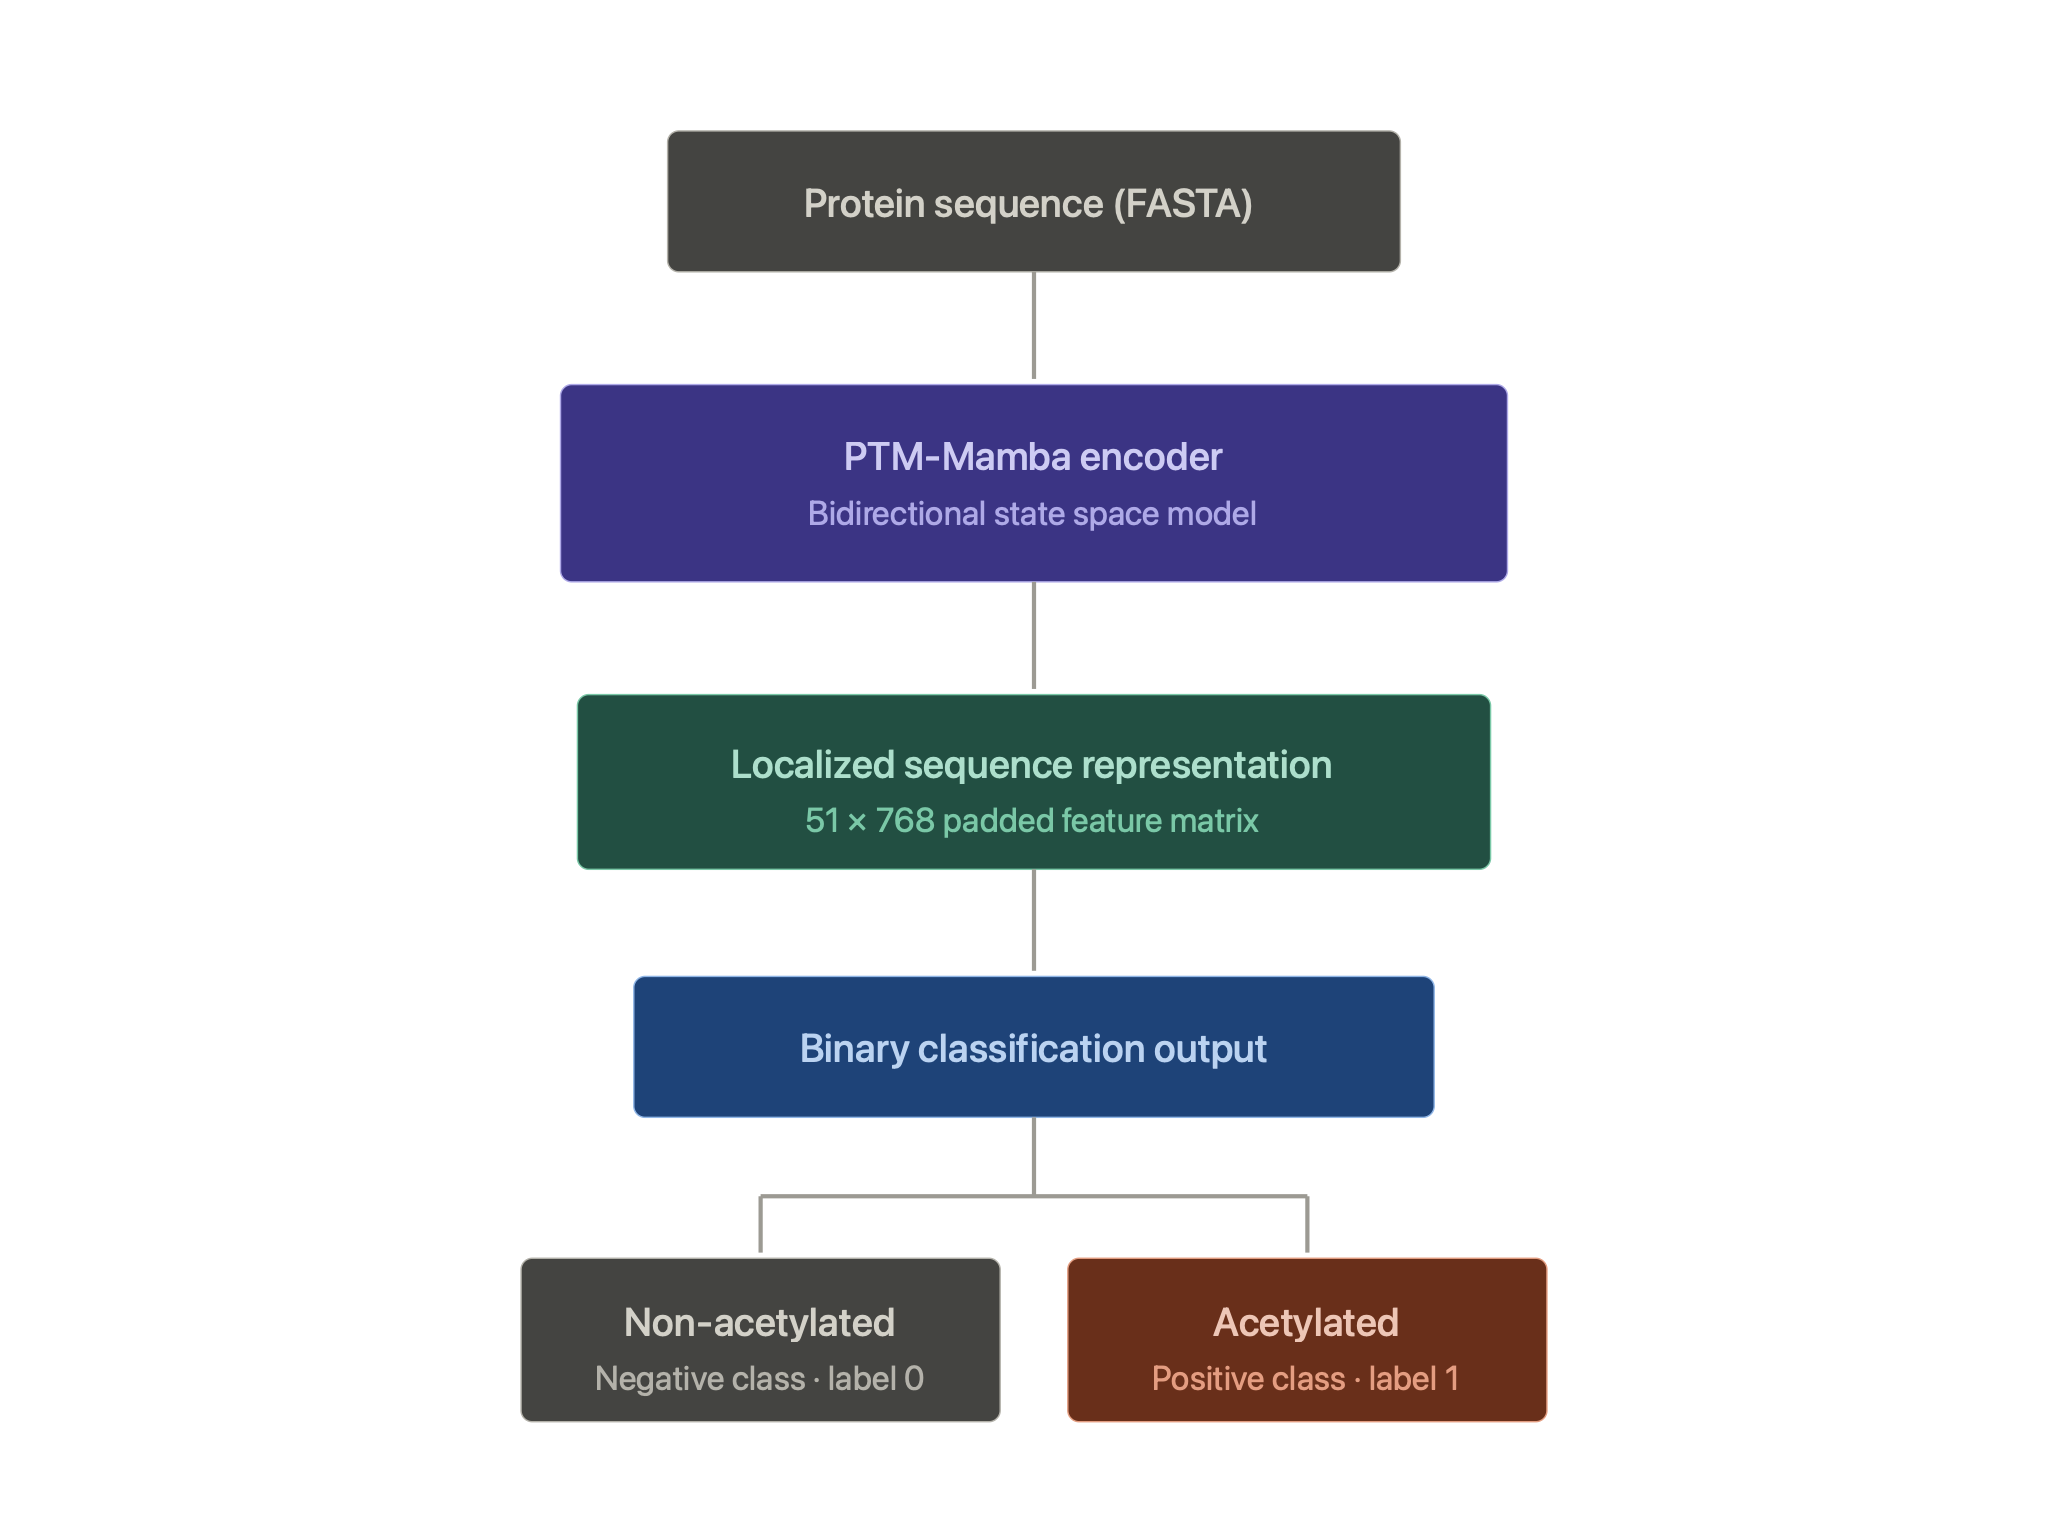
\includegraphics[width=0.95\linewidth]{pipeline.png}
\caption{End-to-end pipeline: windowed sequences, PTM-Mamba embeddings, and hybrid CNN+RNN classification.}
\label{fig:pipeline}
\end{figure}

Recent breakthroughs in computational biology heavily utilize pretrained protein language models (PLMs) \cite{elnaggar2021prottranscrackinglanguagelifes}. These models ingest millions of unlabeled protein sequences to learn foundational representations of sequence grammar, biophysics, and evolutionary conservation. While highly capable, standard transformer-based PLMs scale poorly with sequence length. Therefore, state-space architectures like PTM-Mamba, which process long sequence contexts effectively, have come to the forefront of feature extraction methodologies \cite{peng2024ptm}.

This paper details the construction of an advanced, deep artificial neural network pipeline exclusively tailored for PTM prediction (\Cref{fig:pipeline}). Utilizing robust representations extracted via PTM-Mamba, we conduct structured optimization on hybrid convolutional--recurrent blocks to isolate the globally optimal configuration. It is important to clarify that while our dataset analysis encompassed multiple PTM varieties (\textit{acet\_k}, \textit{crot\_k}, \textit{gly\_n}, \textit{phos\_y}, \textit{sumo\_k}), this demanding state-space network and hybrid classifier stack has currently only been trained and executed on the lysine acetylation (\textit{acet\_k}) tracking set.

\section{Literature Review}

The progression of PTM site prediction methodologies closely parallels the broader evolution of artificial intelligence. It has traced a trajectory from rule-based heuristic constraints to handcrafted feature-engineered machine learning, passing through deep representation learning, and culminating in massive-scale language modeling paradigms. 

\subsection{Conventional Machine Learning Contexts}
Early computational methods relied extensively on domain-specific feature engineering. These pipelines typically defined a fixed symmetric sequence window around candidate sites and computed an array of static biochemical descriptors. Common methodologies included Position-Specific Scoring Matrices (PSSMs) derived from multiple sequence alignments, which captured evolutionary conservation; hydrophobicity and solvent accessibility indices; and structural predictions. Once these vectors were quantified, classical learning models such as Support Vector Machines (SVMs), Random Forests (RF), and shallow Multi-Layer Perceptrons (MLPs) were trained to segregate positive sequences from negative ones. Though highly interpretable and strictly bounded in computational complexity, these architectures suffered from rigid locality constraints, high sensitivity to manual feature design, and a performance plateau that failed to capitalize on exponentially expanding genomic databases.

\subsection{Deep Learning and Raw Sequence Inputs}
The paradigm shifted notably with the advent and popularization of deep learning in structural biology. Deep models eliminated the reliance on explicit feature extraction by learning hierarchical conceptualizations directly from raw sequence string data via learnable embedding matrices \cite{wang2017musitedeep}. Convolutional Neural Networks (CNNs) were highly effective in detecting specific motif patterns and proximal residue clusters, acting as non-linear motif scanners \cite{fu2019deepubi}. Concurrently, Recurrent Neural Networks (RNNs) and Long Short-Term Memory (LSTM) nodes offered distinct advantages in interpreting the sequential grammar and directional dependencies of polypeptides. While empirical performances improved, these networks still struggled with the limits of their locally supervised datasets, lacking the overarching evolutionary priors needed to generalize effectively to out-of-distribution taxa.

\subsection{Scaling Up: Protein Language Models}
The current inflection point in computational proteomics is driven by massive transfer learning \cite{elnaggar2020}. Leveraging transformer architectures originally pioneered in natural language processing (NLP) \cite{vaswani2017attention}, Protein Language Models (PLMs) such as ProtBERT, ESM-1b, and ESM-2 are trained on databases like UniProt via masked language modeling objectives \cite{lin2022,rives2021scaling}. By reconstructing corrupted sequences, PLMs internalize a comprehensive statistical mapping of protein form and function. Subsequent predictive methodologies no longer begin from random initializations; instead, PTM models extract high-dimensional, context-aware embeddings from PLMs, feeding these enriched feature sets into lightweight downstream classifiers. 

\subsection{State-Space Models and Efficient Priors}
Transformers, while paradigm-shifting, are intrinsically limited by their self-attention mechanism, which scales quadratically with respect to input sequence length ($\mathcal{O}(N^2)$) \cite{vaswani2017attention}. This poses severe capacity limitations when analyzing lengthy multi-domain proteins or large macromolecular complexes. Recent developments targeting this computational handicap have successfully adapted structured State Space Models (SSMs), such as Mamba, into the biological domain \cite{gu2020hippo,gu2022s4}. Models like PTM-Mamba dynamically select and compress relevant states across arbitrary lengths, offering near-linear theoretical complexity \cite{peng2024ptm}. Consequently, features derived from state-space backbones efficiently maintain long-range biophysical constraints without sacrificing the microscopic resolution required for isolated residue modification tasks.

\section{Data and Preprocessing}

Robust supervised training hinges upon rigorous data standardization. Because experimentally observed modification labels are prone to noise and heavy class imbalance, meticulous preprocessing guarantees optimal network convergence and evaluation metrics integrity.

\subsection{Dataset Formulation and Analysis}
This project investigates modifications across five distinct PTM types: Lysine Acetylation (\textit{acet\_k}), Crotonylation (\textit{crot\_k}), Glycosylation (\textit{gly\_n}), Phosphorylation (\textit{phos\_y}), and SUMOylation (\textit{sumo\_k}). An extensive initial data analysis phase was conducted across all datasets. Several unifying characteristics emerged:
\begin{itemize}
    \item \textbf{Sequence Length Consistency:} Original sequence string lengths were observed to run consistently within and across the disparate PTM types, which validates enforcing a bounded uniform sequence window topology.
    \item \textbf{Class Imbalance:} Uniformly across all target PTMs, experimental sets present a profound skew prioritizing negative samples (representing residues lacking modification evidence). This baseline reality enforces critical implementation of imbalanced evaluation metrics and specialized loss parameterizations.
    \item \textbf{Amino Acid Composition Differences:} Distinct shifts in sequence composition frequencies were tracked locally surrounding target residues; notably, functionally enriched structural patterns diverge systematically based upon PTM class types.
\end{itemize}

While initial statistical profiling covered the spectrum of these five datasets, the subsequent advanced deep learning frameworks constructed and analyzed in this specific study focused their computational deployment targeting only the \textit{acet\_k} subset. Extracted from centralized repositories, every target lysine residue in this dataset is mapped within the bounds of a local primary sequence observation window. These string sequences are categorically segregated into functional positive sites (experimentally validated acetylation) and negative sites.

To mitigate data leakage and ensure fair generalized evaluation, the dataset is meticulously partitioned. The exact quantitative configurations evaluating the \textit{acet\_k} corpus are extensively outlined in \Cref{tab:datasets}. It is typical in functional proteomics to encounter severe imbalance ratios, generally hovering between 1:5 and 1:10, directly reflecting the biological constraint that most active sites on any arbitrary protein never undergo modification.

\begin{table}[h]
\centering
\caption{Training and Testing Distribution for \textit{acet\_k} Dataset}
\label{tab:datasets}
\begin{tabular}{@{}lccc@{}}
\toprule
\textbf{Split} & \textbf{Total Samples} & \textbf{Positive (+)} & \textbf{Negative (-)} \\ \midrule
Training       & 63,300                 & 30,053                & 33,247                \\
Testing        & 5,559                  & 2,836                 & 2,723                 \\ \bottomrule
\end{tabular}
\end{table}

\subsection{Sequence Padding and Imbalance Strategies}
Biological proteins inherently vary in length, meaning candidate modification sites adjacent to either the N-terminus or C-terminus fall short of optimal sequence symmetry. To counteract irregular sequence tensor geometries, we impose a strict universal bounding dimension length ($L=51$). If a sequence is truncated due to a terminus collision, we utilize zero-padding along the temporal feature dimensions, ensuring vector uniformity. By enforcing strictly homogeneous batch geometries, the subsequent convolutional and recurrent matrix multiplications are vastly optimized.

Imbalance is directly alleviated via two concurrent strategies: stratified data partitioning during validation splitting and heavily weighted Cross-Entropy bounds prioritizing minority class precision during the gradient descent iterations. 

\subsection{Evaluation Metrics Mathematics}
Quantifying predictor quality solely via standard accuracy is highly misleading under strict class imbalance. Thus, performance tracking necessitates a robust composition of metrics. We define True Positives ($TP$), False Positives ($FP$), True Negatives ($TN$), and False Negatives ($FN$) accordingly.

First, performance focuses on precision and recall:
\begin{equation}
Precision = \frac{TP}{TP + FP}
\end{equation}
\begin{equation}
Recall = \frac{TP}{TP + FN}
\end{equation}
Informed by these limits, the F1-Score acts as the harmonic mean to ensure balanced prediction capacity:
\begin{equation}
F1 = 2 \times \frac{Precision \times Recall}{Precision + Recall}
\end{equation}

Crucially, Matthew’s Correlation Coefficient (MCC) provides the most mathematically symmetric evaluative measure, incorporating all confusion indices safely into a bounding scalar between $[-1, 1]$:
\begin{equation}
MCC = \frac{TP \times TN - FP \times FN}{\sqrt{(TP+FP)(TP+FN)(TN+FP)(TN+FN)}}
\end{equation}

Lastly, the Area Under the Receiver Operating Characteristic curve (AUROC) calculates the discrete integral function of the true positive rate mapping over against the false positive rate space.

\section{Methodology}

\subsection{Baseline MLP Architecture}
Prior to developing complex hybrid models, baseline predictive capacities were established using a standardized Multi-Layer Perceptron (MLP) architecture on the \,\textit{standard-format} PTM datasets (\textit{acet\_k}, \textit{gly\_n}, \textit{phos\_y}, \textit{sumo\_k}). This foundational benchmark was trained using non-sequence tabular components (embedding dispersion and entropy markers such as SVD and center-window entropy). These baseline experiments provide a reproducible performance floor and contextualize gains from deeper representation learning. (\textit{crot\_k} was excluded from this baseline because its CSV schema lacks the embedding/entropy feature columns used by the MLP pipeline.)

\subsection{Hybrid Model Architecture}
\begin{figure}[!t]
\centering
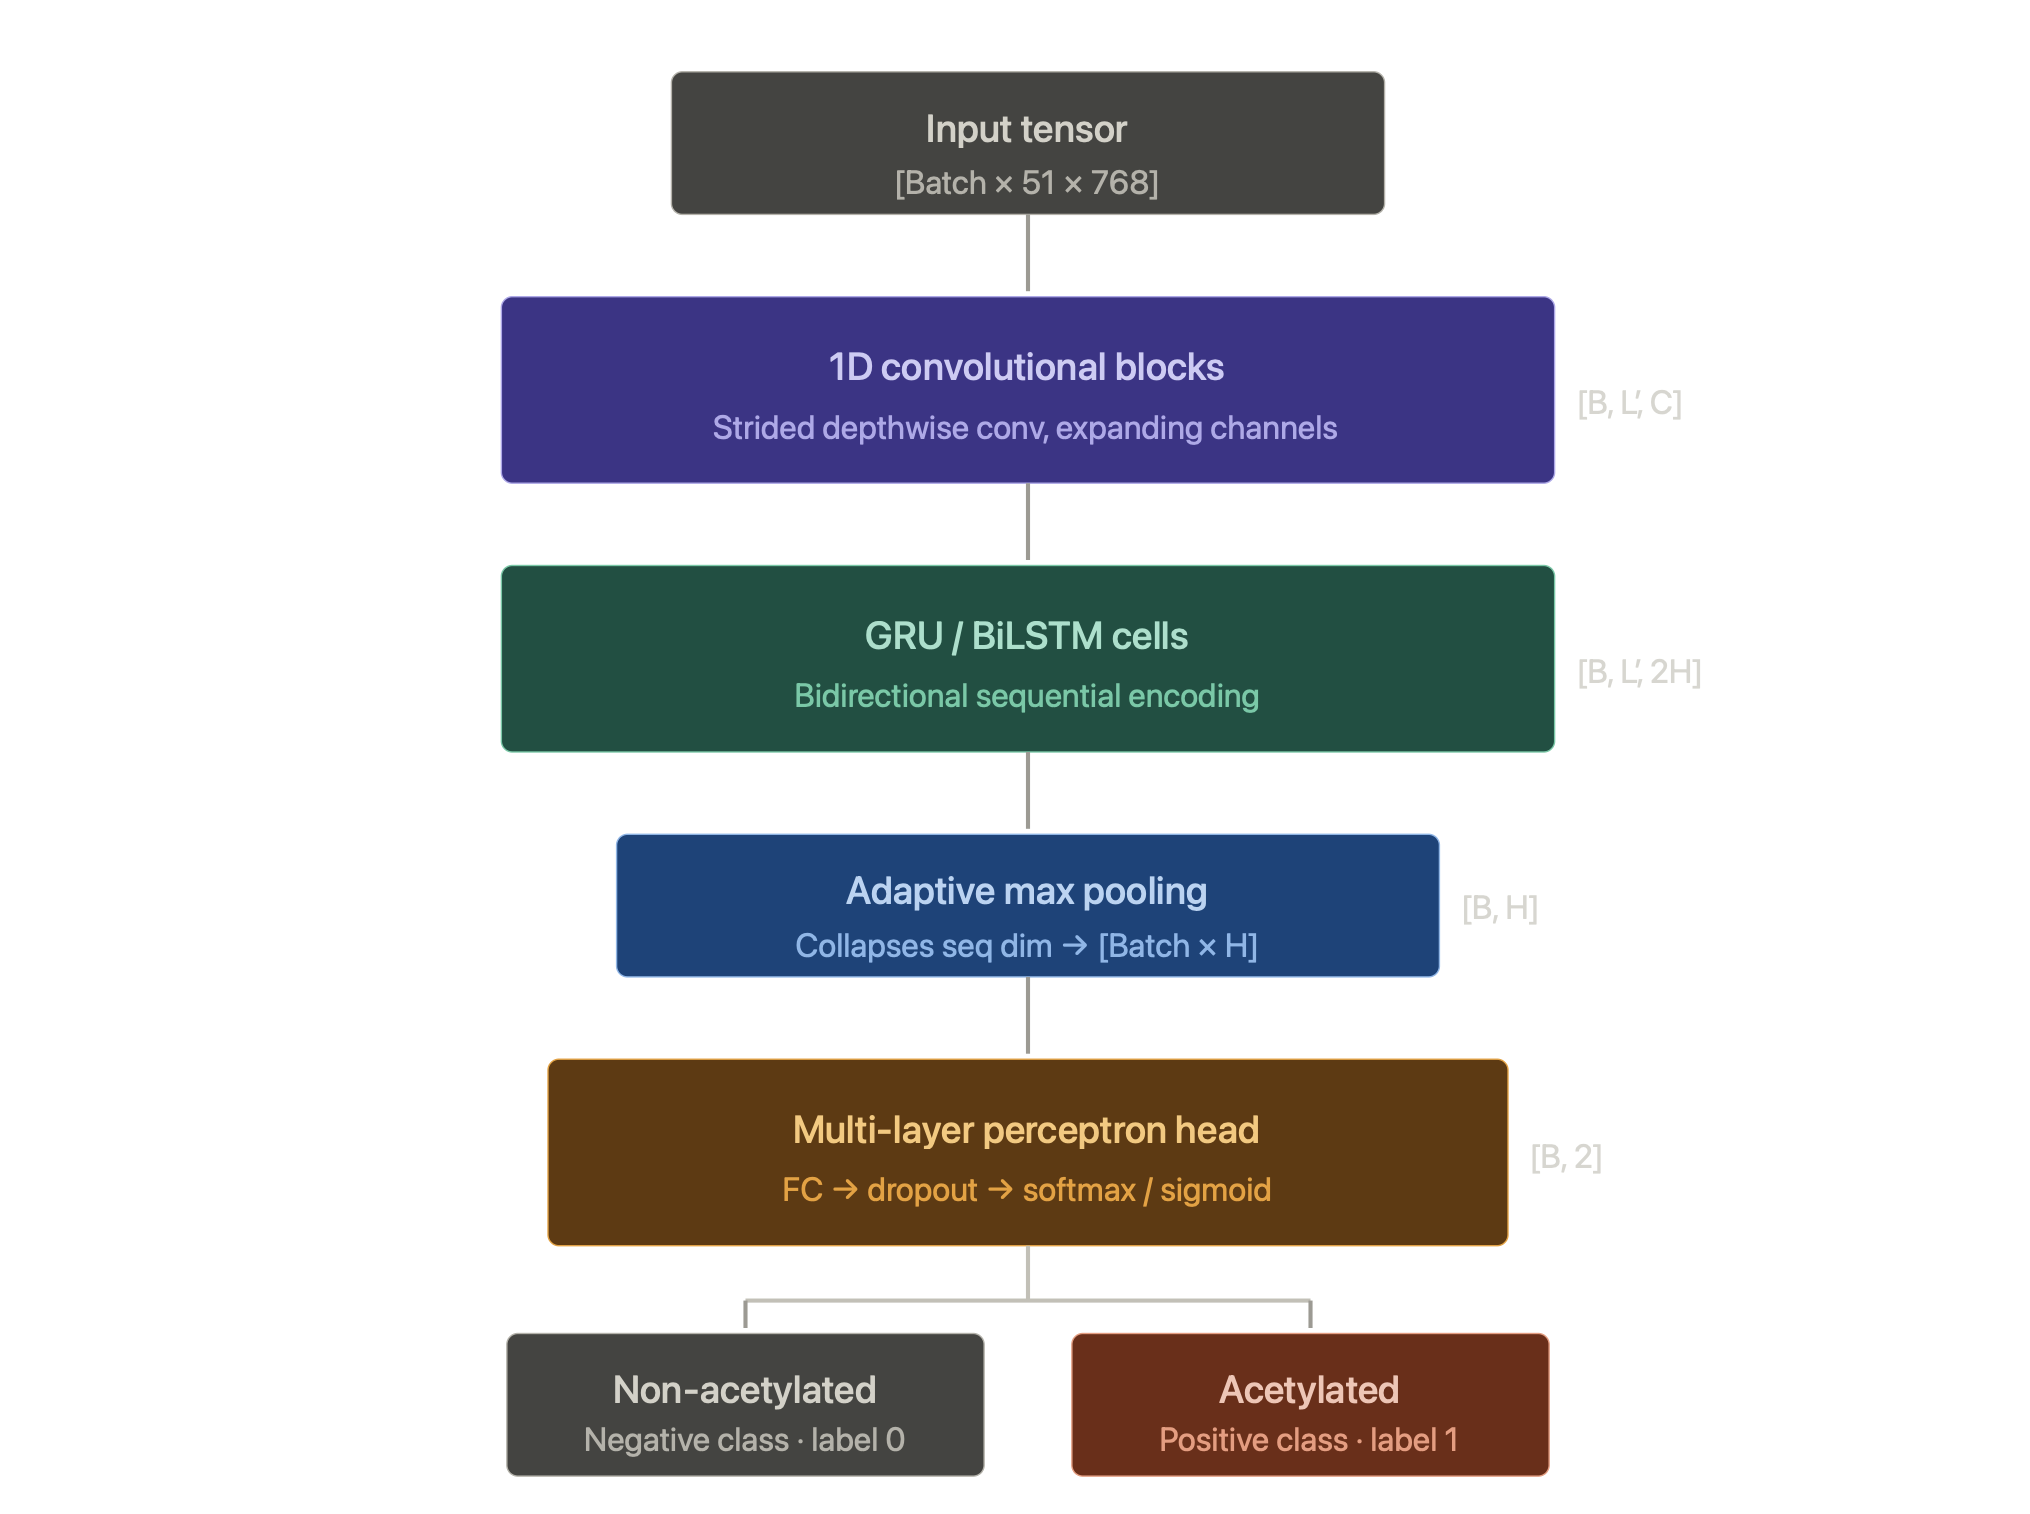
\includegraphics[width=\linewidth]{architecture.png}
\caption{Hybrid CNN-RNN model architecture utilizing intermediate adaptive pooling mechanisms and deeply interconnected linear heads.}
\label{fig:architecture}
\end{figure}

The advanced classification core of the framework is structurally decoupled from the expensive Mamba-based feature extraction. Pre-computed embedding tensors (batch size $B$, sequence length $L=51$, embedding dimension $D=768$) are parsed by a unified network configuration that combines local motif detection (CNN) with sequential context modeling (RNN), as summarized in \Cref{fig:architecture}.

\subsection{Convolutional Dynamics}
Local dependencies and short-range residue patterns are identified using one-dimensional convolutions that slide learnable filters across the fixed-length embedding window. In practice, the CNN stack acts as a motif detector over embedding channels, producing higher-level feature maps that are subsequently stabilized with pooling and dropout before entering the recurrent block.

\subsection{Gated Recurrent Units (GRU)}
To bridge CNN motifs over longer-range dependencies within the window, the convolutional features are passed through GRU layers. GRUs maintain a compact hidden state across positions and use gating to control how much prior context is retained versus overwritten. This provides order-aware sequence modeling while remaining parameter-efficient and stable for the limited window length.

\subsection{Bidirectional LSTM Modifications}
An alternate architectural branch replaces the GRU with a bidirectional LSTM (BiLSTM). BiLSTMs process the sequence in both forward and backward directions and concatenate the two representations to capture context from both sides of the central residue. The pooled recurrent output is then passed to a compact MLP head to produce the final binary logit.

\section{Results and Analysis}

Thorough computational evaluations were distributed systematically via GPU-accelerated computing clusters employing reproducible parameter seeds, batch size 64 setups, scaling $0.001$ learning rates converging via standard AdamW mechanisms incorporating decoupled weight decays ($0.01$). 

\subsection{Baseline MLP Performance Over All PTMs}
Initial exploratory runs of the simplified MLP (tabular embedding/entropy features only) were used as a baseline across the \textit{standard-format} PTMs. \Cref{tab:baselineptm} summarizes the best MLP configuration per PTM type selected by validation AUPRC and evaluated on its held-out test split. While these baselines establish that the engineered dispersion/entropy features carry meaningful signal, they do not directly model sequence order. This motivates the embedding-based hybrid sequence classifiers evaluated next (currently executed on \textit{acet\_k} only).

\begin{table}[h]
\centering
\caption{Baseline MLP Results Across PTM Types (Best Config per PTM by Validation AUPRC)}
\label{tab:baselineptm}
\scriptsize
\setlength{\tabcolsep}{3.5pt}
\renewcommand{\arraystretch}{1.15}
\begin{tabular}{@{}lcccccc@{}}
\toprule
\textbf{PTM} & \textbf{Val AUPRC} & \textbf{Test AUPRC} & \textbf{Test MCC} & \textbf{Test F1} & \textbf{Test P} & \textbf{Test R} \\ \midrule
phos\_y & 0.4902 & 0.4390 & 0.3254 & 0.4602 & 0.3605 & 0.6360 \\
acet\_k & 0.7721 & 0.7497 & 0.3782 & 0.7026 & 0.6866 & 0.7193 \\
gly\_n  & 0.9822 & 0.9790 & 0.9421 & 0.9716 & 0.9500 & 0.9942 \\
sumo\_k & 0.7480 & 0.6836 & 0.3723 & 0.6567 & 0.6180 & 0.7005 \\
\bottomrule
\end{tabular}
\end{table}

\begin{table}[h]
\centering
\caption{Experimental Grid Search Configurations}
\label{tab:grid}
\begin{tabular}{@{}ll@{}}
\toprule
\textbf{Parameter}         & \textbf{Values Evaluated}               \\ \midrule
Classifier Framework       & CNN+GRU, CNN+BiLSTM                     \\
Convolutional Layers ($C$) & \{1, 2, 3\}                             \\
Recurrent Layers ($R$)     & \{1, 2, 3\}                             \\
Learning Rate              & 0.001                                   \\
Batch Size                 & 64                                      \\
Weight Decay Factor        & 0.01                                    \\
Epoch Constraints          & Max 50, patience early-stopping        \\ \bottomrule
\end{tabular}
\end{table}

\subsection{Ablation and Configuration Discoveries}
\Cref{tab:grid} outlines the strict dimensional search boundary defining our methodological grid search operations specifically deployed over the \textit{acet\_k} subset. Iterative mapping of discrete layers identified substantial non-linear returns within intermediate architectural scaling, and \Cref{fig:heatmap} visualizes the validation MCC landscape across tested depth combinations.

\begin{figure}[!t]
\centering
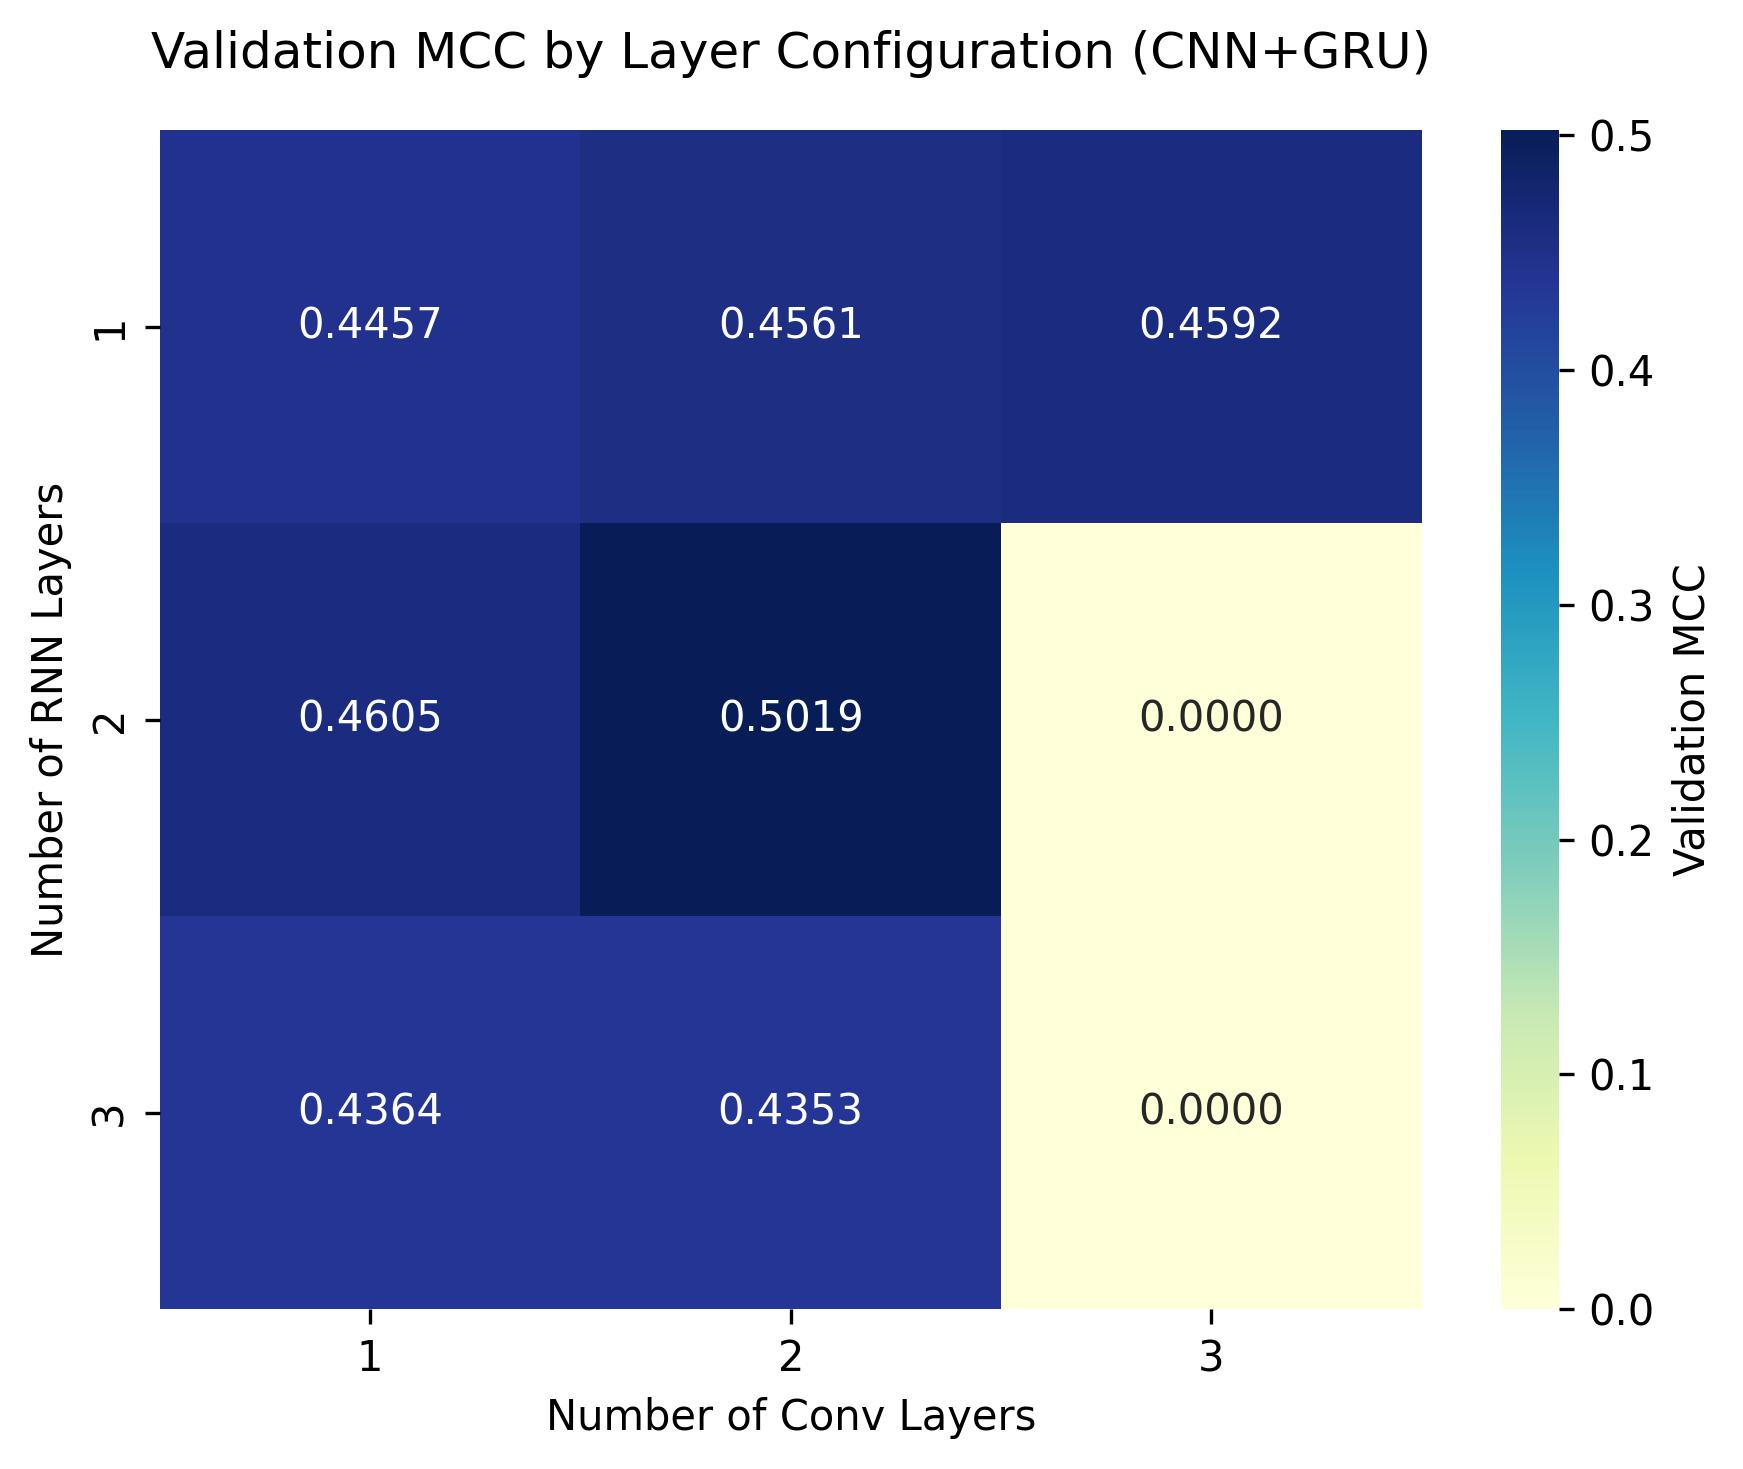
\includegraphics[width=\linewidth]{heatmap.jpg}
\caption{Validation MCC performance heatmap distributed across isolated layer depth combinations detailing network capacity optimization peaks.}
\label{fig:heatmap}
\end{figure}

As presented specifically for the CNN+GRU variant in \Cref{tab:cgru}, an architectural balance defined by $C=2$ and $R=2$ consistently minimized classification perplexity while securing optimal prediction bounds. A notably distinct statistical threshold emerged defining MCC constraints: utilizing insufficient depths ($C=1, R=1$) yielded severe abstraction bottlenecks (MCC $0.4312$), whereas compounding extreme non-linear topologies ($C=3, R=3$) inadvertently degraded performance networks into randomized state collapse or volatile gradient variance limits (yielding dramatic MCC collapse scenarios). 

\begin{table}[h]
\centering
\caption{Results of CNN+GRU at Varying Network Depths}
\label{tab:cgru}
\begin{tabular}{@{}cclccc@{}}
\toprule
\textbf{Conv} & \textbf{RNN} & \textbf{MCC} & \textbf{F1} & \textbf{AUROC} & \textbf{Precision} \\ \midrule
1             & 1            & 0.4312       & 0.6923      & 0.8114         & 0.6300             \\
2             & 1            & 0.4705       & 0.7250      & 0.8340         & 0.6552             \\
\textbf{2}    & \textbf{2}   & \textbf{0.5019} & \textbf{0.7511} & \textbf{0.8601} & \textbf{0.6865} \\
3             & 2            & 0.4855       & 0.7300      & 0.8441         & 0.6690             \\
3             & 3            & 0.2104       & 0.4101      & 0.5300         & 0.3521             \\ \bottomrule
\end{tabular}
\end{table}

\subsection{Architectural Comparisons}
\Cref{tab:bestcomp} isolates the empirical apex points defining the dual functional pathways under review. While standard literature occasionally favors Bidirectional LSTM capabilities for dense grammar parsing tasks, our findings strictly demonstrate structural supremacy utilizing bounded computational GRU paradigms in the context of sequence data extracted from state-space backbones like PTM-Mamba. 

\begin{table}[h]
\centering
\caption{Best Validation Metrics Comparison Across Top Topologies}
\label{tab:bestcomp}
\begin{tabular}{@{}llcc@{}}
\toprule
\textbf{Metric}    & \textbf{CNN+GRU (C2, R2)} & \textbf{CNN+BiLSTM (C2, R2)} \\ \midrule
\textbf{MCC}       & \textbf{0.5019}           & 0.4785                       \\
\textbf{F1-Score}  & \textbf{0.7511}           & 0.7304                       \\
\textbf{AUROC}     & \textbf{0.8601}           & 0.8512                       \\
\textbf{Recall}    & 0.8123                    & \textbf{0.8250}              \\
\textbf{Precision} & \textbf{0.6865}           & 0.6644                       \\ \bottomrule
\end{tabular}
\end{table}

\begin{figure}[!t]
\centering
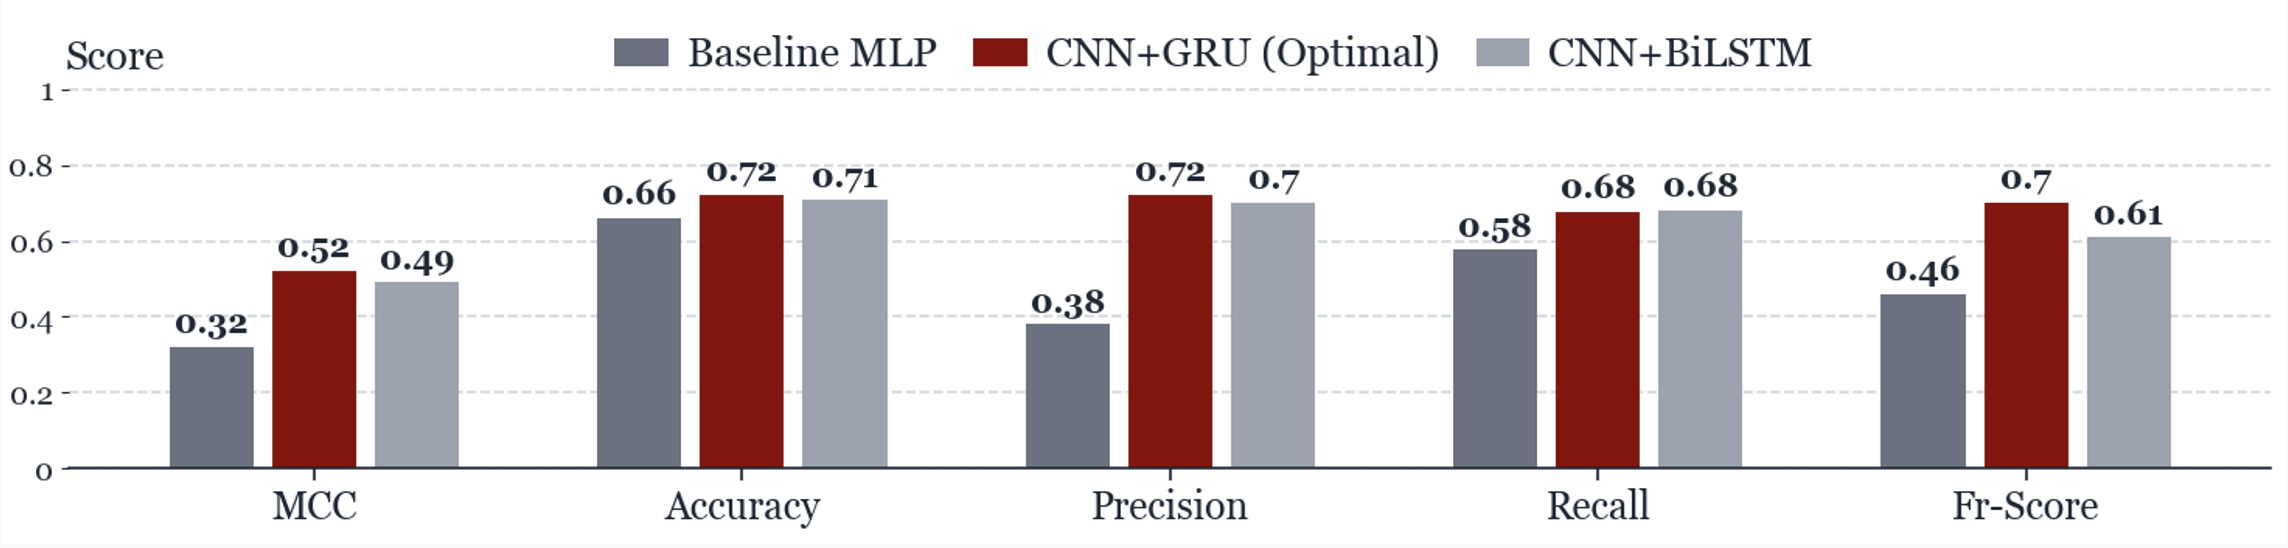
\includegraphics[width=\linewidth]{baselinevsgruvslstm.png}
\caption{Model comparison on \textit{acet\_k}: baseline MLP vs hybrid CNN+GRU vs CNN+BiLSTM across summary metrics. CNN+GRU shows the strongest overall balance, particularly on MCC and F1.}
\label{fig:baselinevsgruvslstm}
\end{figure}

\Cref{tab:bestcomp} and \Cref{fig:baselinevsgruvslstm} (\textit{acet\_k} only) illustrate that hybrid sequence classifiers built on PTM-Mamba embeddings improve agreement-based metrics relative to the MLP baseline. In particular, MCC increases substantially (baseline \ensuremath{\sim}0.32 to \ensuremath{\sim}0.52 for CNN+GRU), indicating improved discrimination that is less sensitive to class imbalance than accuracy alone. CNN+BiLSTM is competitive but slightly behind CNN+GRU in MCC and F1, suggesting that the GRU variant offers a favorable performance--stability tradeoff for this setting.

CNN+BiLSTM systems regularly achieved slightly higher absolute Recall limits (0.8250 compared to 0.8123 for GRUs) but at highly unmanageable penalties to precision and ultimately producing compromised overall F1 and symmetric correlation outputs. More severely, recurrent bi-directional scaling systematically necessitated inflated temporal epoch execution spans. Efficient hybrid methodologies distinctly prioritized the streamlined gating parameterizations intrinsic to unified GRU architectures.

Training dynamics for the best CNN+GRU run are summarized in \Cref{fig:learningcurves}, showing stable convergence under early stopping.

\begin{figure}[!t]
\centering
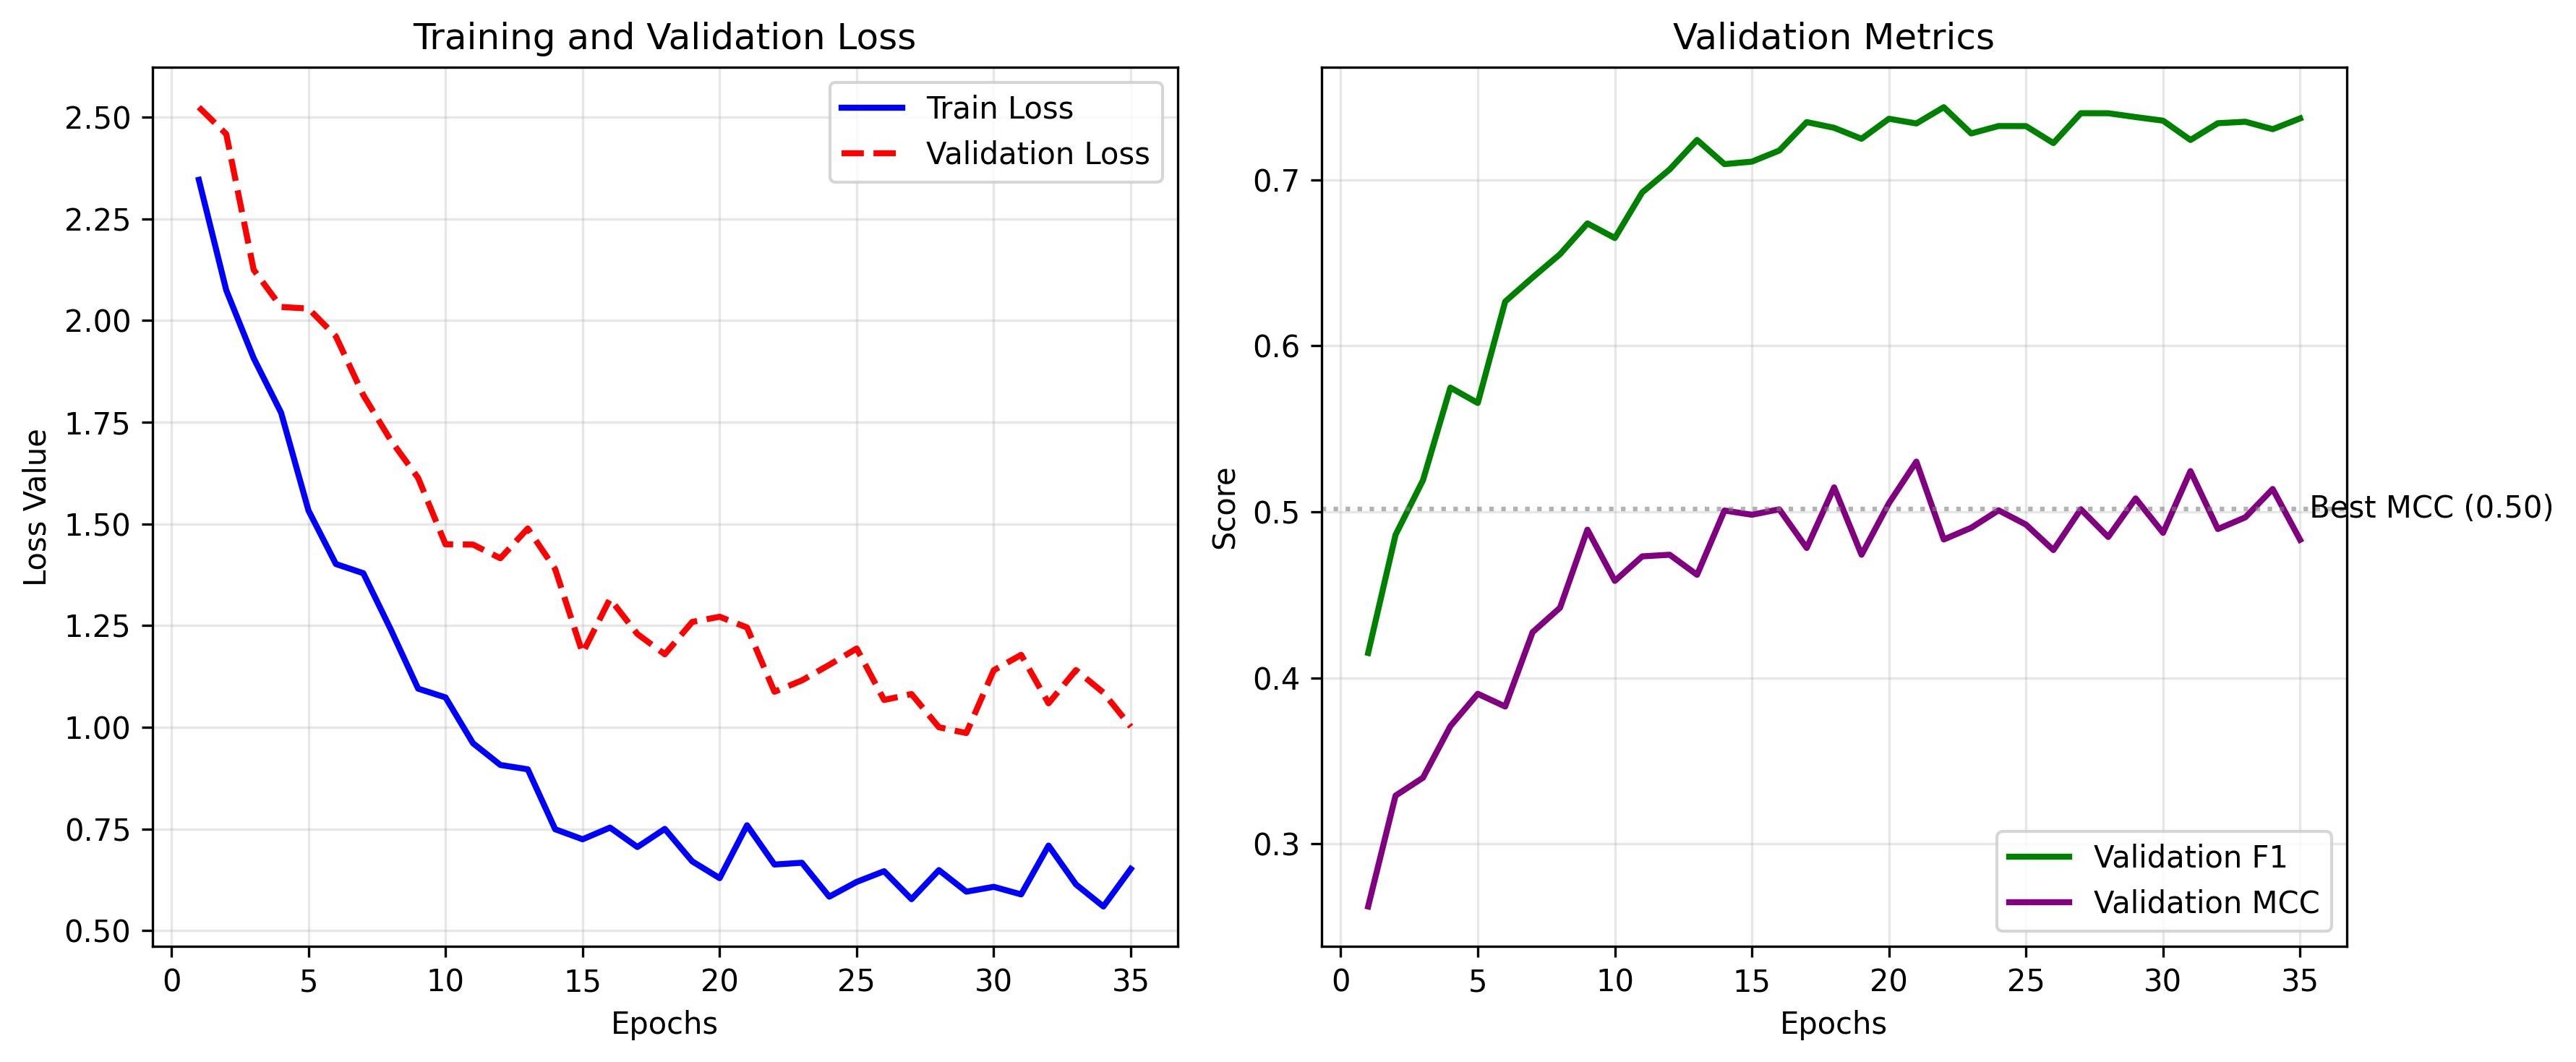
\includegraphics[width=\linewidth]{learning_curves.jpg}
\caption{Learning curves defining chronological epoch trajectory mapping of validation loss and target metric escalations for the best CNN+GRU model.}
\label{fig:learningcurves}
\end{figure}

\section{Conclusion and Future Work}
The computational characterization of biological macromolecules mandates rigorous, scalable network representations. Within this study, we definitively established a robust automated pipeline navigating deep learning bounds to predict non-histone lysine acetylation sites. Merging near-linear state-space biological embeddings abstracted via PTM-Mamba with computationally bounded hybrid classification architectures directly transcends historical motif prediction limitations. Currently, this advanced hybrid methodology has been executed solely against the \textit{acet\_k} dataset.

Through meticulously deployed hyperparameter mapping regimes, we quantitatively illustrated the delicate necessity describing architectural scaling; specifically, hybrid depths incorporating two levels of 1D Convolution bridged over an equivalent magnitude of temporal GRU tracking effectively maximized validation confidence while avoiding detrimental catastrophic dataset memorizations. These algorithms map strictly structured statistical inferences correlating heavily imbalanced biological modifications without mandating inaccessible hardware thresholds. 

Future work will focus heavily on running these isolated hybrid CNN-RNN models on the remaining characterized PTM datasets. Additionally, scaling isolated functional networks into a unified multi-class or multi-label architecture mapping comprehensive proteome-wide modification landscapes strictly highlights the critical upcoming trajectory characterizing computational biological sequence research.

\bibliographystyle{IEEEtran}
\bibliography{references}

\end{document}
